\chapter{Traffic Setting Descriptions}

\section{Vehicle Volume Counting Locations}
\label{section:traffic_descriptors}

This section of the report describes the different locations used for testing the volume counting functionality of the system's computer vision algorithm. At the end of the section images of each location are included.

\textbf{Location 1}: 

\begin{itemize}
    \item Bi-directional six-lane traffic.
    \item Camera angle is moderately high. 
    \item Many shadows cast by low-angle sun.
    \item High volume traffic of large variety, features many semi-trailers. 
    \item Camera perspective in-line with traffic direction.
\end{itemize}
 

\textbf{Location 2}:

\begin{itemize}
    \item One direction of four-lane traffic.
    \item Moderately high camera angle.
    \item Large shadows from low-angle sun.
    \item Tree a lot of movement from trees in background.
    \item Traffic completely stops at times.
    \item Vehicles appearing from mid-frame in merging lane on far right.
    \item Camera perspective in-line with traffic direction.
\end{itemize}


\textbf{Location 3}: 

\begin{itemize}
    \item Bidirectional eight-lane traffic.
    \item High volume and high speed vehicles.
    \item Moderate camera angle.
    \item Camera occasionally moves.
    \item Vehicles entering and exiting frame at different latitudes depending on the lane.
    \item Overcast day, no shadowing. 
    \item Camera perspective in-line with traffic direction.
\end{itemize}


\textbf{Location 4}:

\begin{itemize}
    \item Bi-directional six-lane traffic.
    \item Camera angle moderately high but off centre.
    \item High angle sun causing minimal shadowing.
    \item Variety of vehicle types including many motorcycles.
    \item High volume traffic.
    \item Traffic comes to complete stop.
    \item Camera perspective in-line with traffic direction.
    \item Large amounts of vehicles occluding each other due to camera angle.
\end{itemize}


\textbf{Location 5}:

\begin{itemize}
    \item Bidirectional four-lane traffic.
    \item Low camera angle.
    \item Camera perspective perpendicular to traffic direction.
    \item Partial lane occlusion due to signage.
    \item Overcast with minimal shadowing.
\end{itemize}


\textbf{Location 6}:

\begin{itemize}
    \item Bidirectional two-lane traffic.
    \item Flat camera angle.
    \item Camera perspective perpendicular to traffic direction.
    \item Overcast with minimal shadowing.
\end{itemize}

\textbf{Location 7}:

\begin{itemize}
    \item Bidirectional two-lane traffic.
    \item High camera angle.
    \item Night time with artificial lighting.
    \item Traffic comes to complete stop.
    \item Partial occlusion of traffic lanes due to signage.
\end{itemize}


\begin{figure}[H]
	\centering
	\begin{subfigure}[b]{0.45\linewidth}
        \centering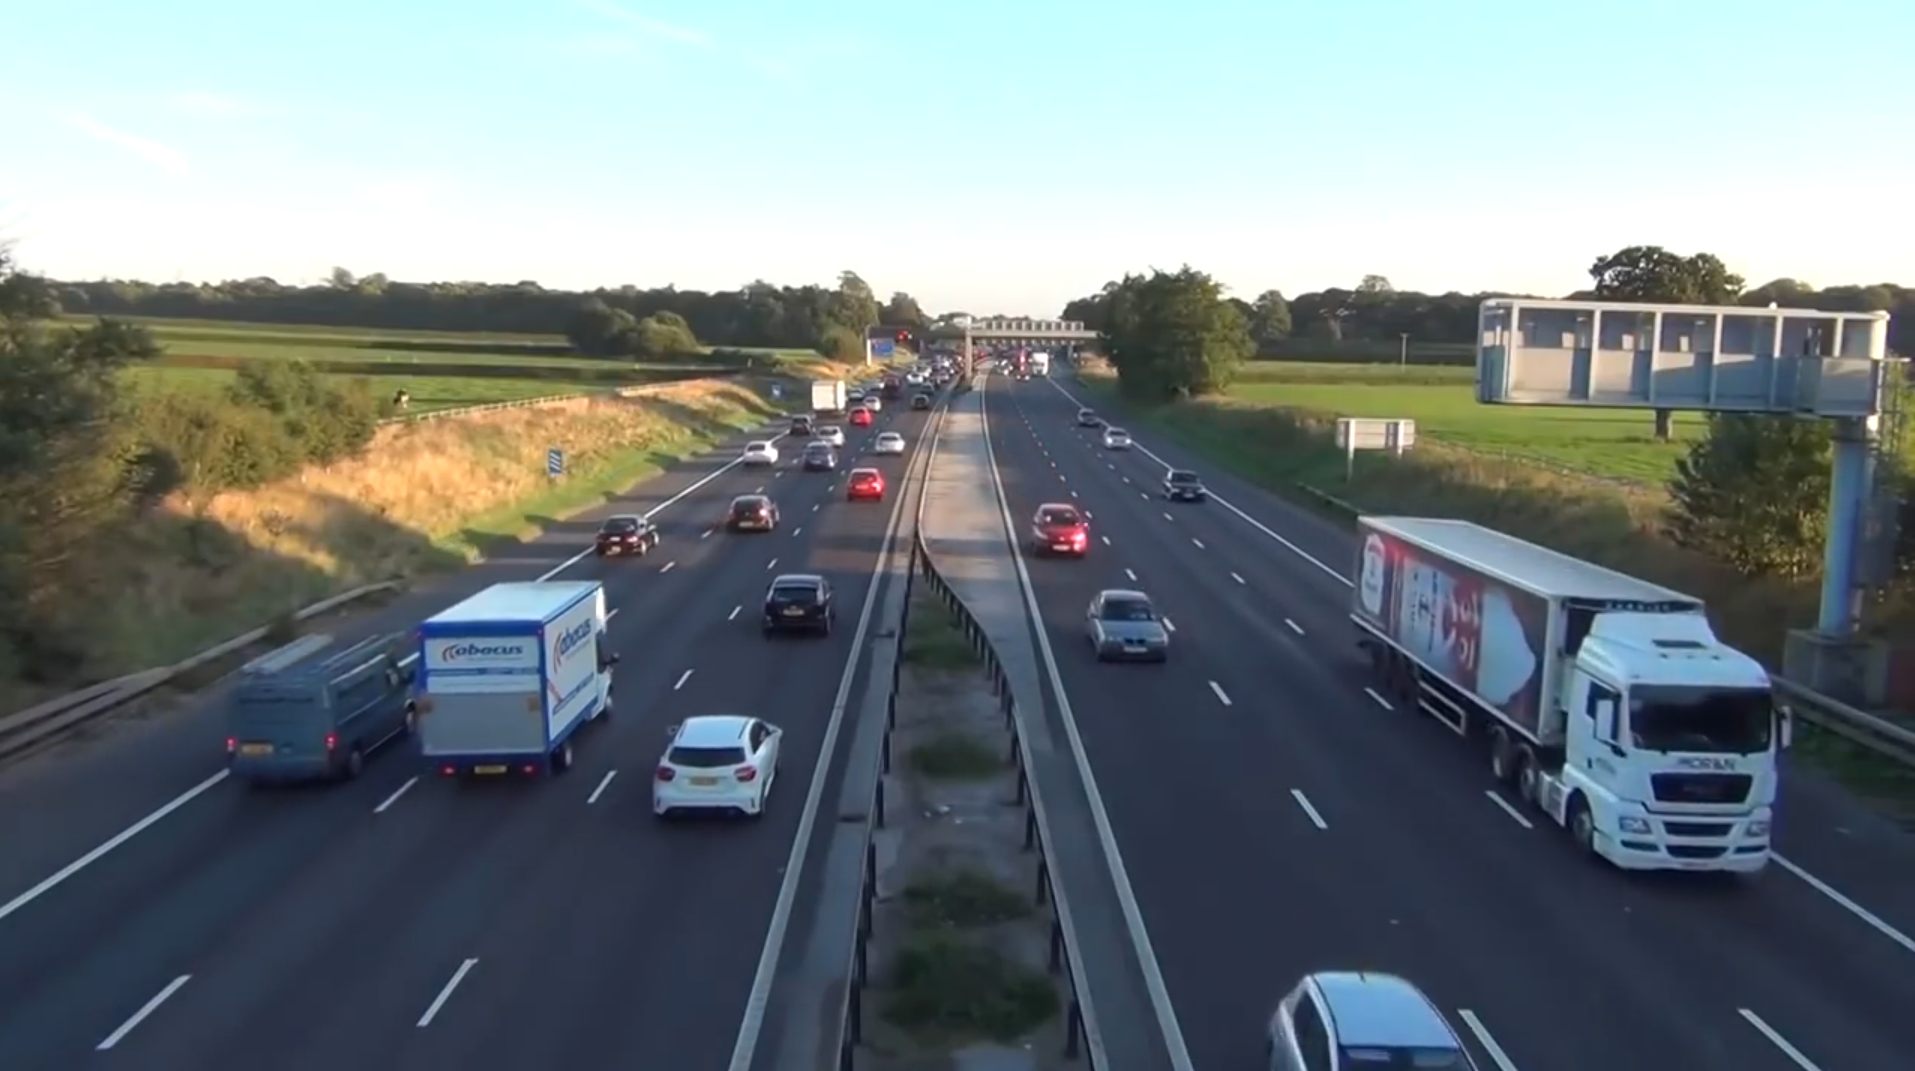
\includegraphics[width = \textwidth]{appendices/descriptors/location_one.png}
        \caption{Location 1}
		\label{fig:location_one}
    \end{subfigure}
    \begin{subfigure}[b]{0.45\linewidth}
        \centering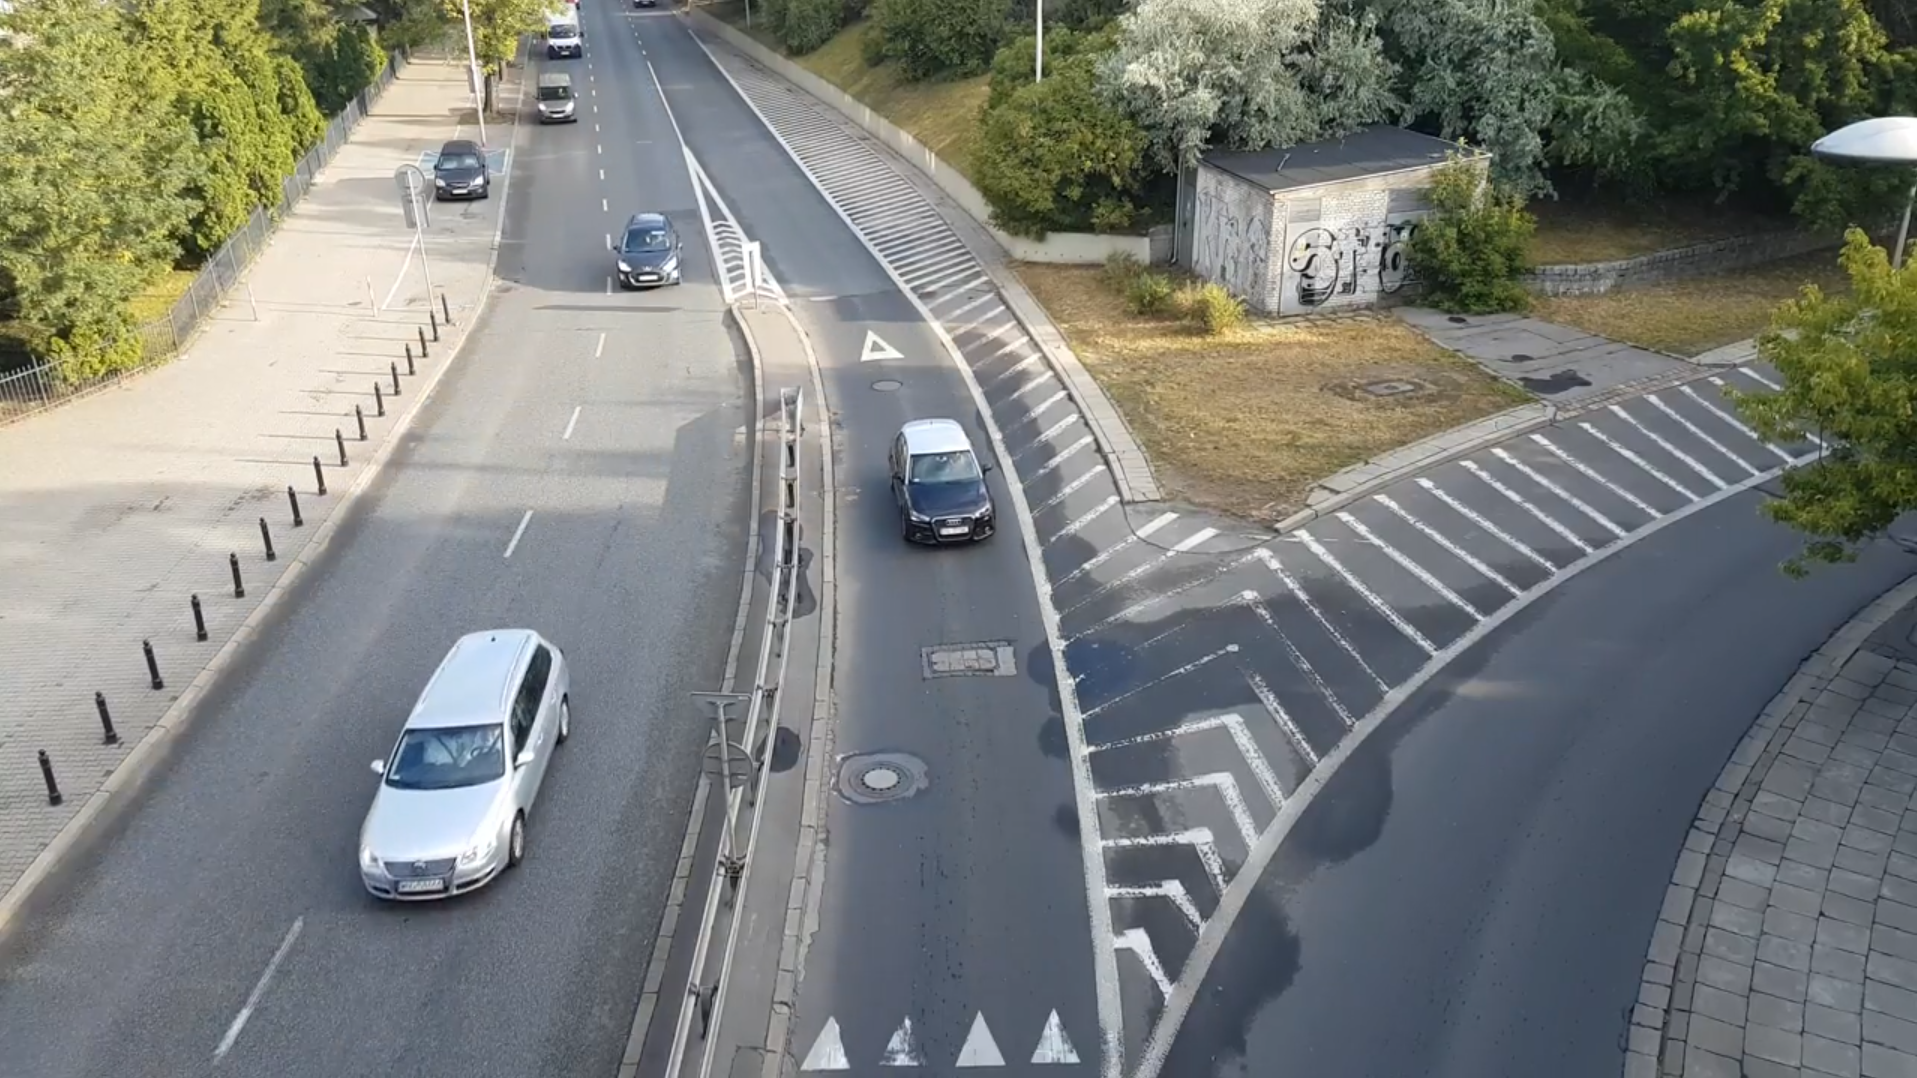
\includegraphics[width = \textwidth]{appendices/descriptors/location_two.png}
        \caption{Location 2}
        \label{fig:location_two}
    \end{subfigure}
    \begin{subfigure}[b]{0.45\linewidth}
        \centering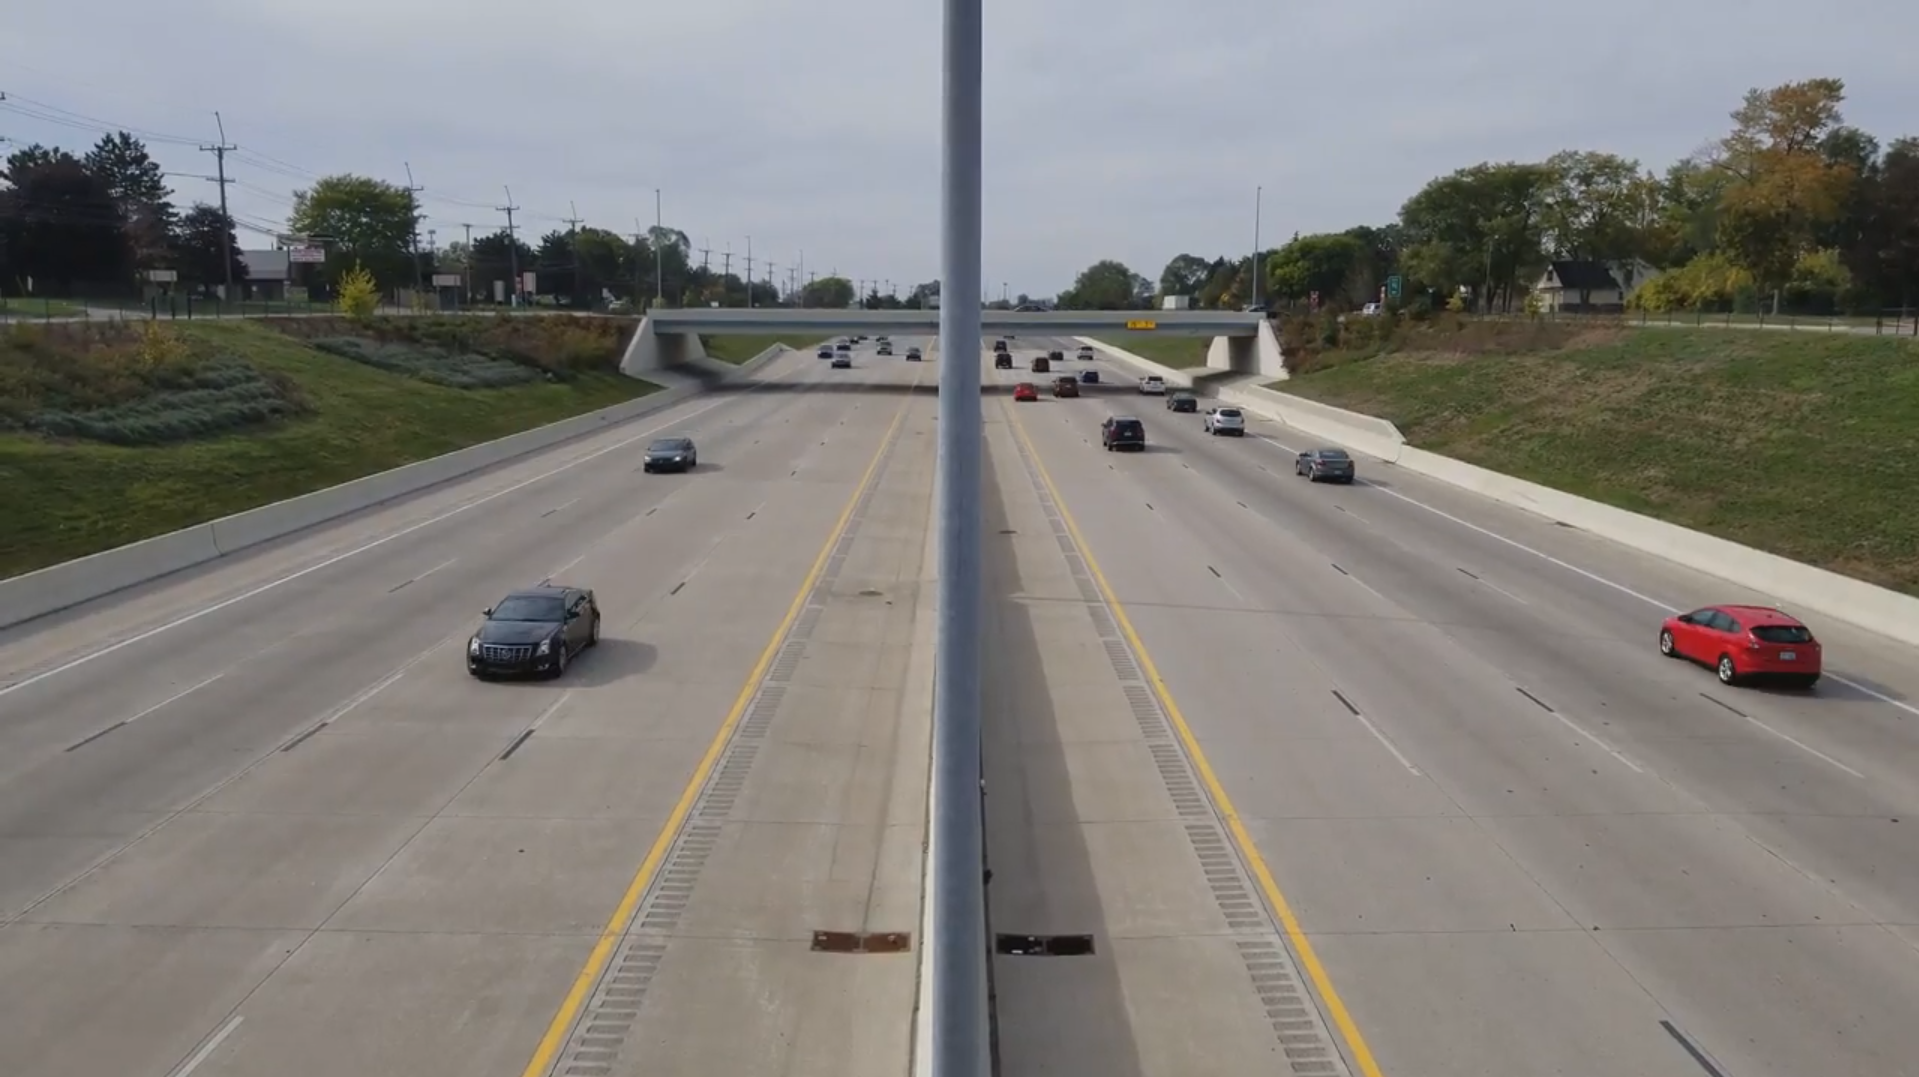
\includegraphics[width = \textwidth]{appendices/descriptors/location_three.png}
        \caption{Location 3}
        \label{fig:location_three}
    \end{subfigure}
    \begin{subfigure}[b]{0.45\linewidth}
        \centering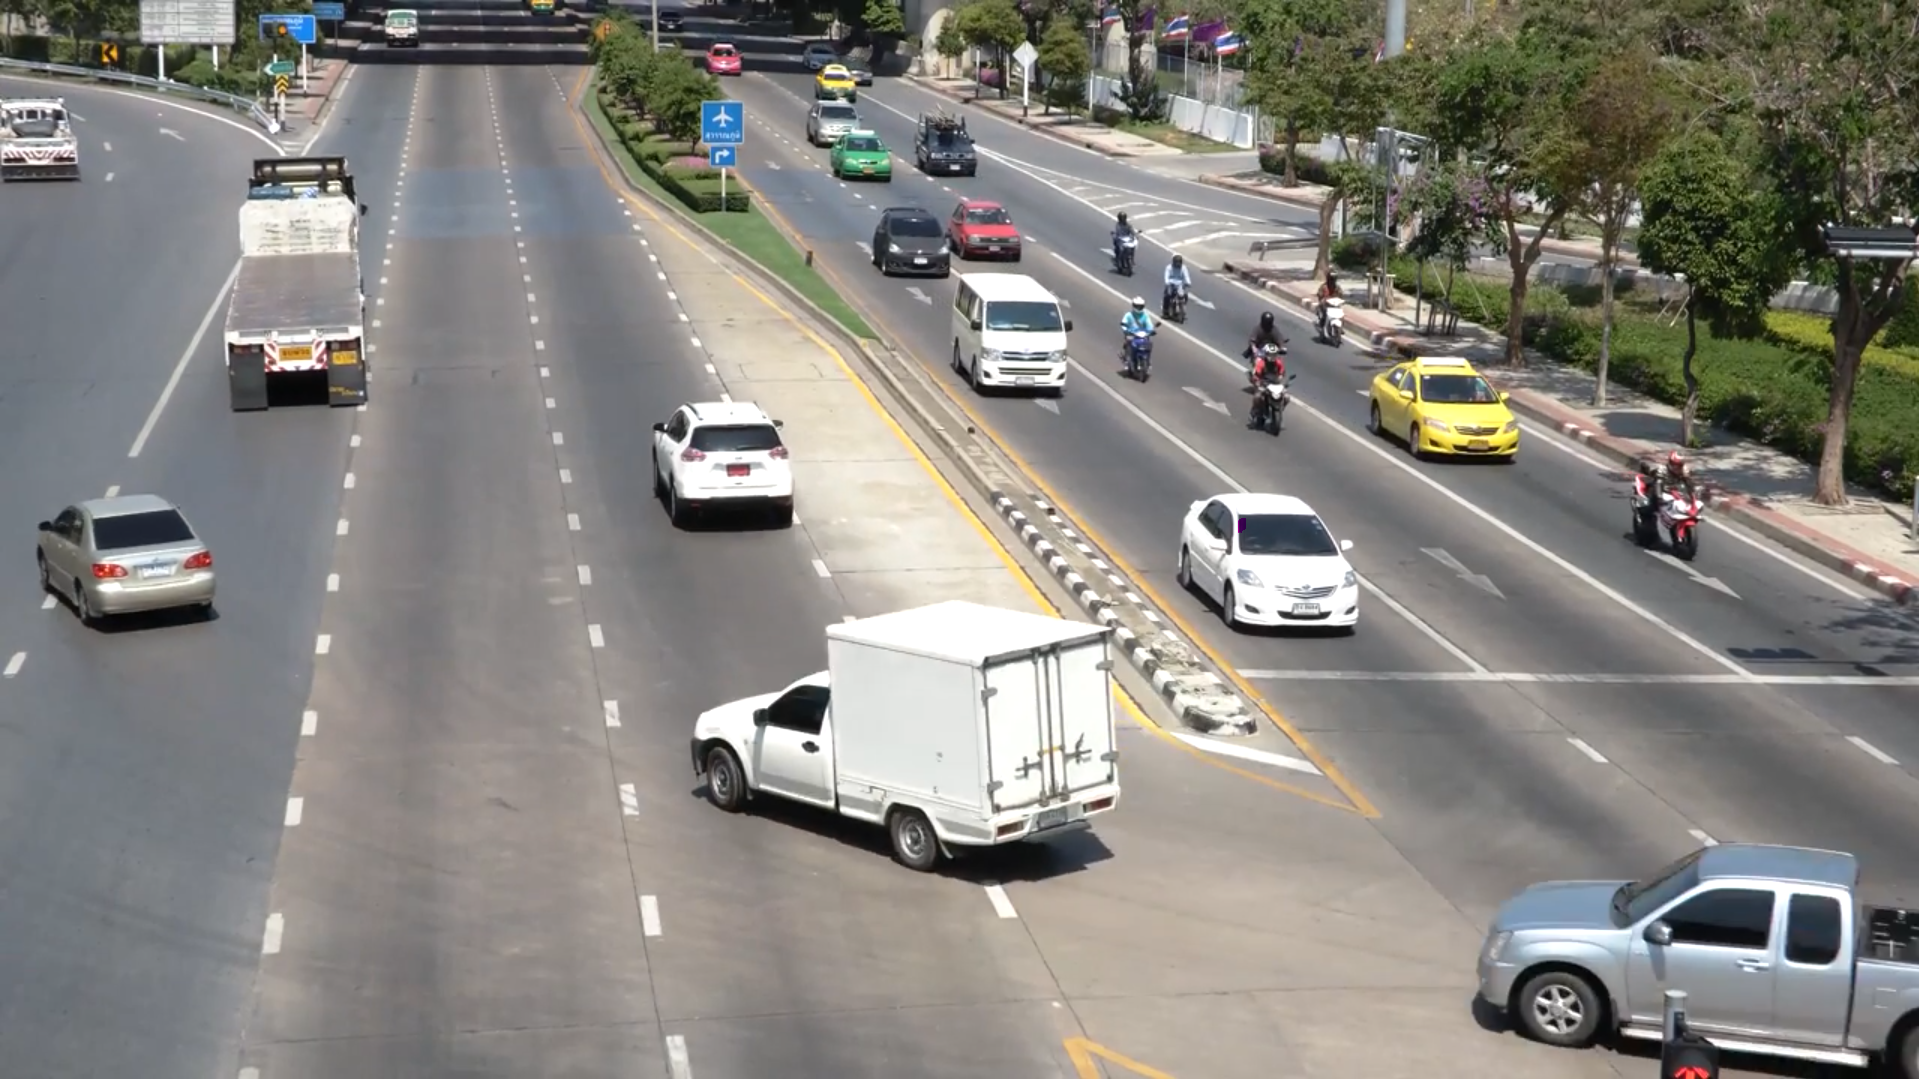
\includegraphics[width = \textwidth]{appendices/descriptors/location_four.png}
        \caption{Location 4}
        \label{fig:location_four}
    \end{subfigure}
    \begin{subfigure}[b]{0.45\linewidth}
        \centering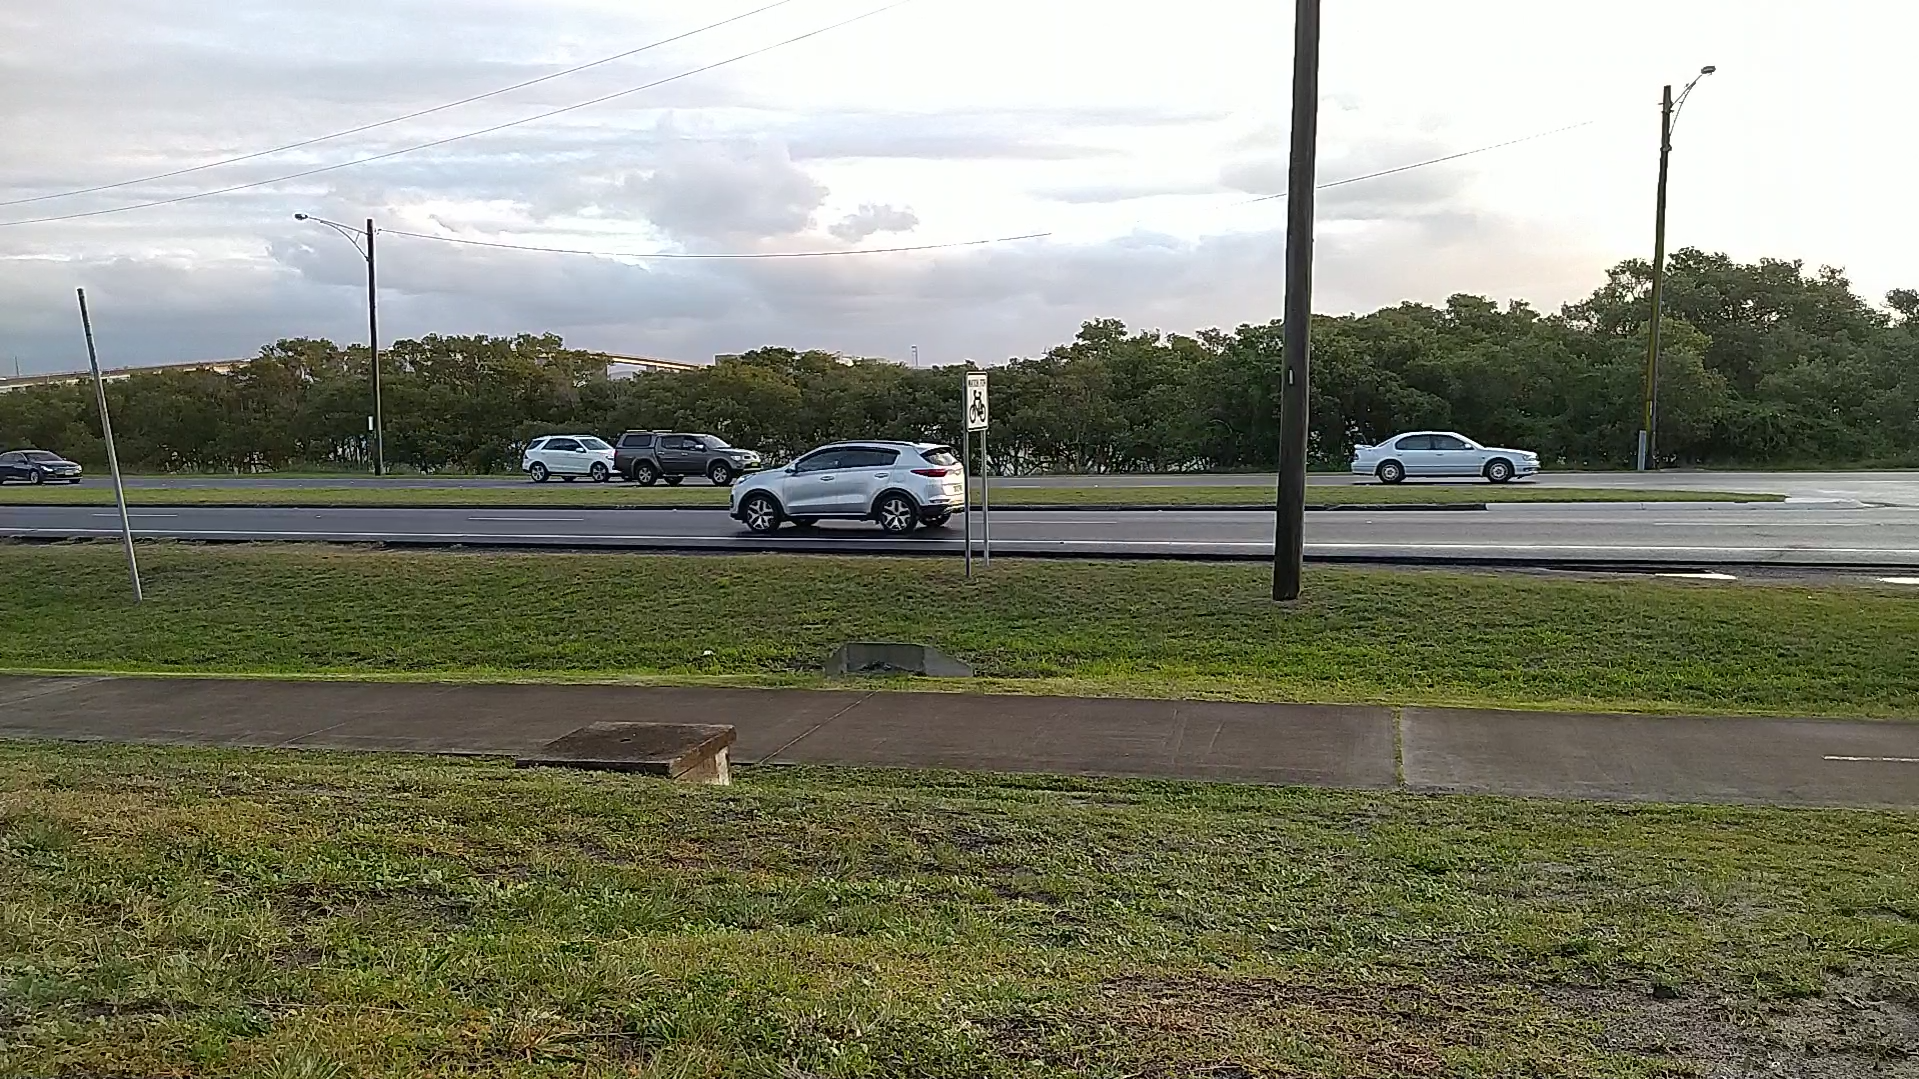
\includegraphics[width = \textwidth]{appendices/descriptors/location_five.png}
        \caption{Location 5}
        \label{fig:location_five}
    \end{subfigure}
    \begin{subfigure}[b]{0.45\linewidth}
        \centering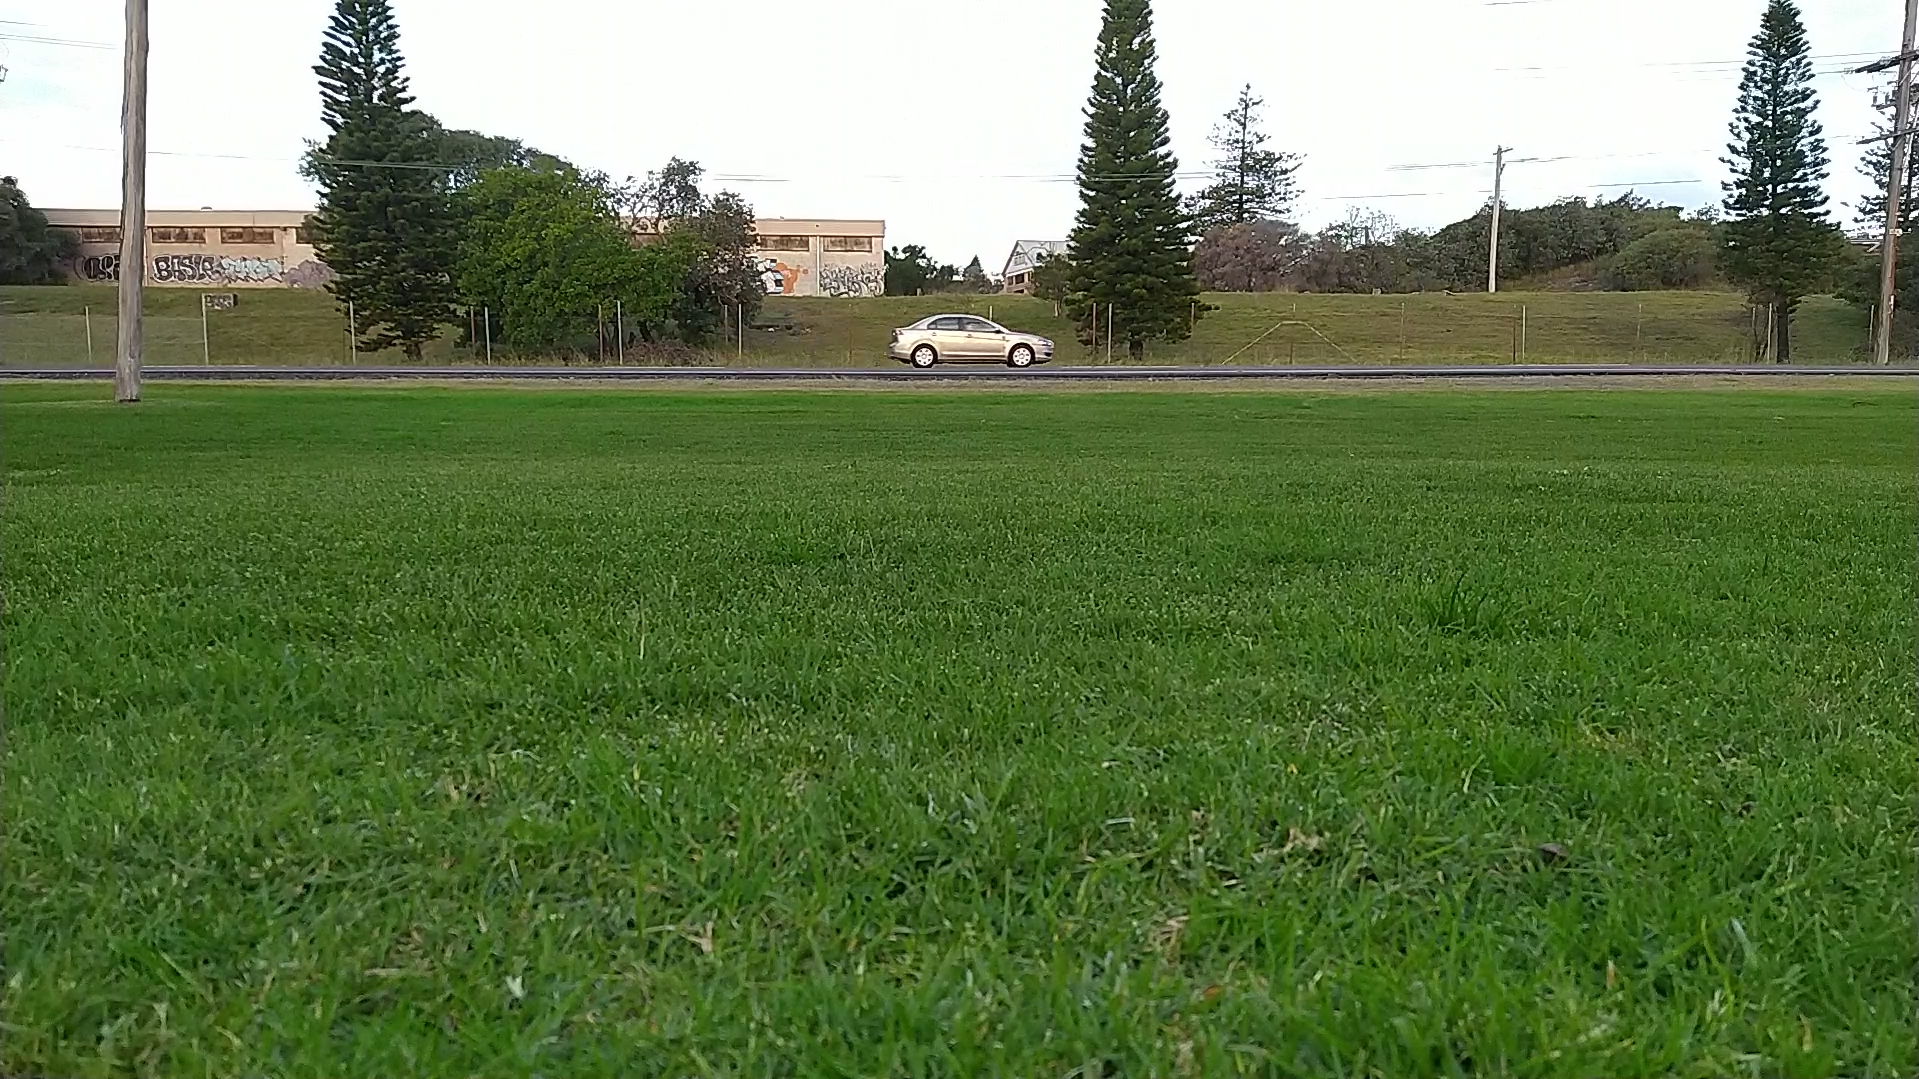
\includegraphics[width = \textwidth]{appendices/descriptors/location_six.png}
        \caption{Location 6}
        \label{fig:location_six}
    \end{subfigure}
    \begin{subfigure}[b]{0.45\linewidth}
        \centering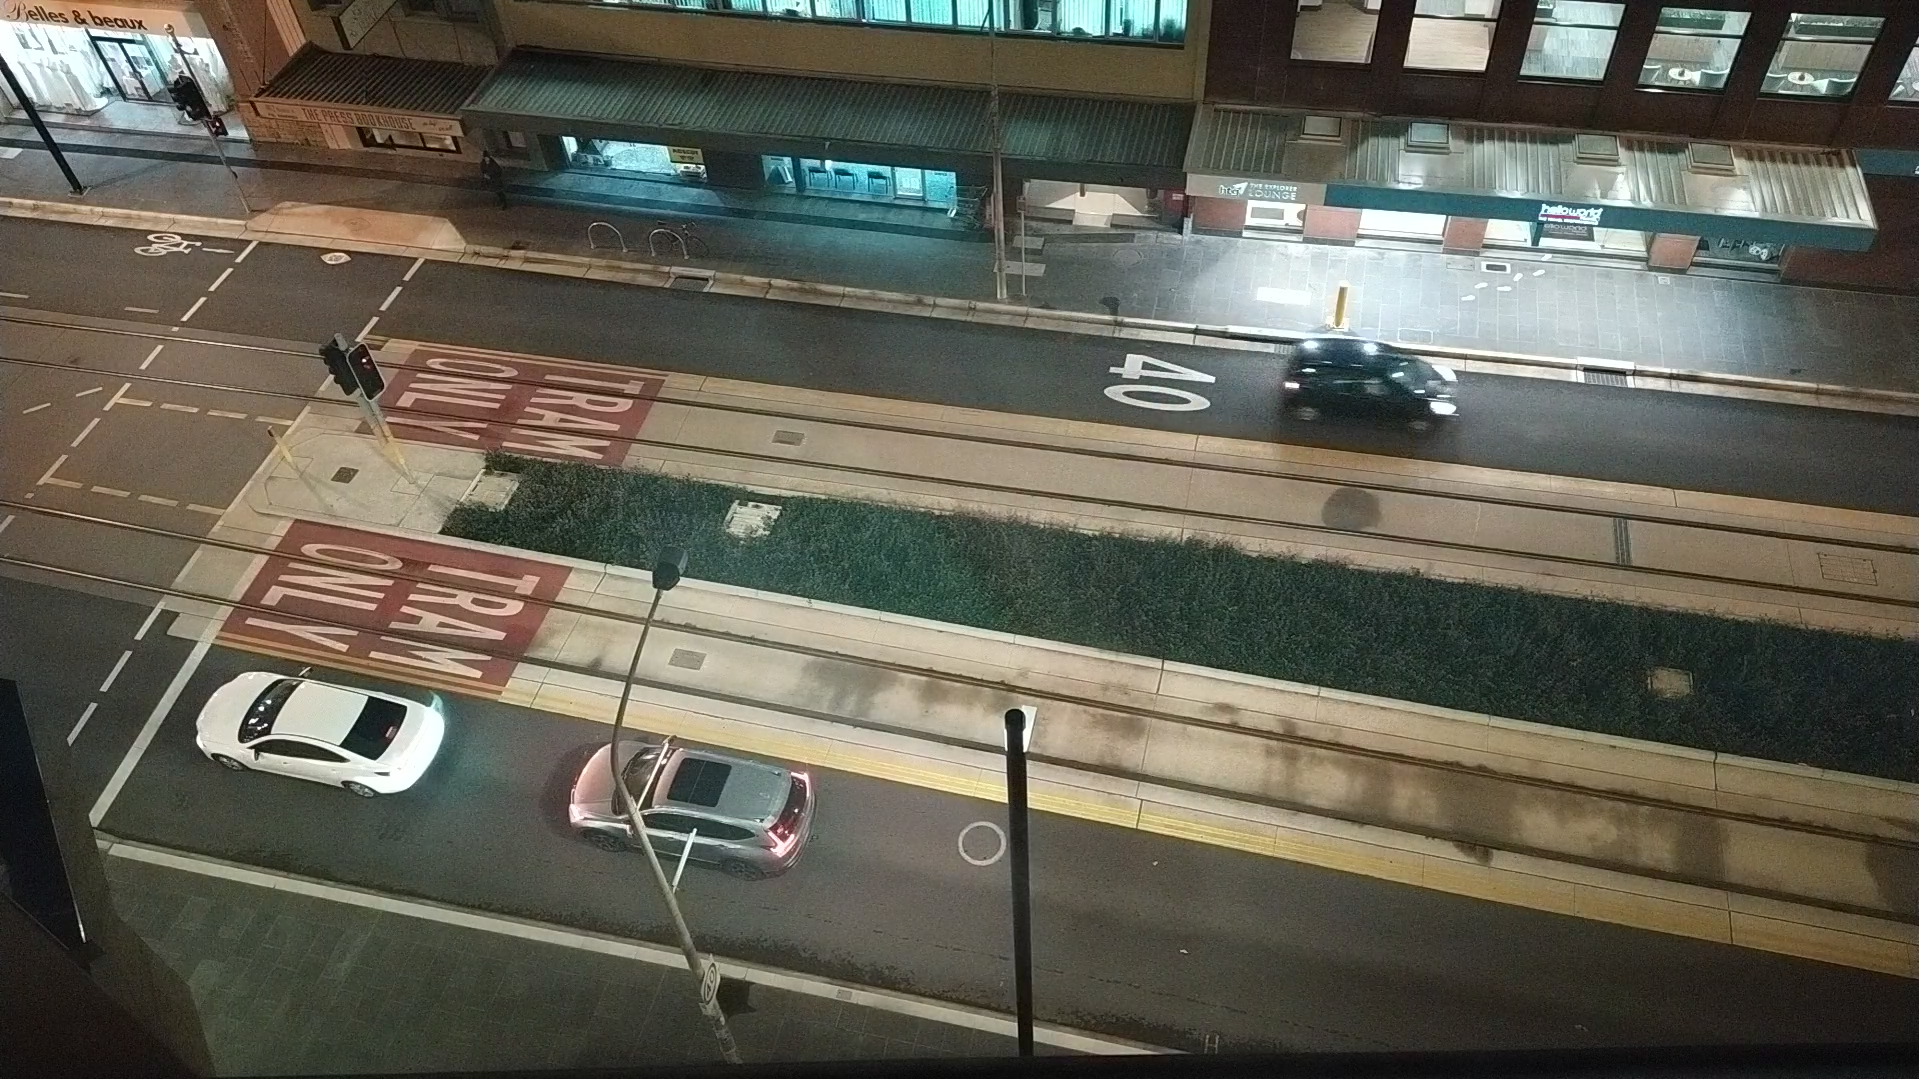
\includegraphics[width = \textwidth]{appendices/descriptors/location_seven.png}
        \caption{}
        \label{fig:location_seven}
    \end{subfigure}
\caption{Traffic testing location snapshots.}
\label{fig:location_snapshots}
\end{figure}